\documentclass{article}
\title{統計学入門 — データの記述から推測統計まで}
\author{TeX 図書館}

\begin{document}

\section{データと統計の考え方}

統計学は\textbf{データから知識を取り出す}ための学問です。この教科書では、データを要約する記述統計から、標本から母集団を推し量る推測統計までを学びます。

\subsection{母集団と標本}

統計の基本的な枠組みは次の2つの世界に分かれます。

\begin{itemize}
\item \textbf{母集団}: 調べたい対象の全体。理想的には全部は観測できない。
\item \textbf{標本}: 実際に観測した一部のデータ。
\end{itemize}

選挙の世論調査が典型です。有権者全員(母集団)に聞くことはできないので、無作為に選んだ数千人(標本)から全体の支持率を推測します。「一部から全体を推測する」ことには必ず誤差が伴い、その誤差を\textbf{確率論}で定量化するのが推測統計の骨格です。

\subsection{変量の種類}

データの型によって適切な分析方法が変わります。
\begin{itemize}
\item \textbf{質的変量(カテゴリ)}: 血液型、性別、商品カテゴリなど。集計は度数と割合。
\item \textbf{量的変量(数値)}: 身長、価格、滞在時間など。平均・分散・分布の形で要約。
\end{itemize}

\begin{quote}
\textbf{【注意】}\ 郵便番号や電話番号は数値に見えますが、大小に意味がないので質的変量です。「平均の電話番号」を計算しても意味がありません。データ型の見極めは分析の第一歩です。
\end{quote}

\section{1変量データの要約}

\subsection{代表値}

量的データの中心を表す代表値には、主に3つあります。

\textbf{平均値}(算術平均):
\[ \bar{x} = \frac{1}{n} \sum_{i=1}^{n} x_i \]

\textbf{中央値}: データを小さい順に並べたときの中央の値。

\textbf{最頻値}: 最も多く現れる値。

\begin{quote}
\textbf{【例】}\ 5人の年収(万円)が \(300, 350, 380, 400, 2600\) だとします。平均は \(\frac{4030}{5} = 806\) 万円ですが、中央値は \(380\) 万円。1人の超大金持ちが平均を大きく引き上げており、分布が歪んでいるときは\textbf{中央値のほうが実感に合う}代表値です。
\end{quote}

使い分けの指針: 分布が左右対称に近ければ平均、歪んでいれば中央値が頑健です。平均はすべてのデータの情報を使う利点がある一方、外れ値に敏感という弱点をもちます。

\begin{figure}[h]
\centering
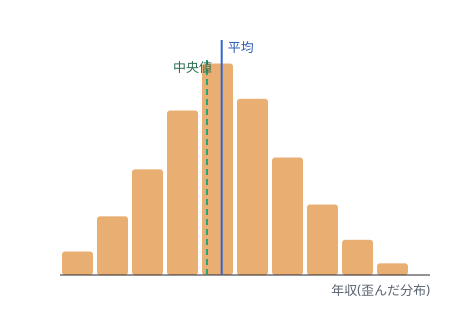
\includegraphics[width=0.7\textwidth]{figures/skewed-hist.svg}
\caption{右に歪んだ分布では、大きい値の一部が平均を中央値より右へ引き上げる。}
\end{figure}

\subsection{散らばりの尺度}

中心だけではデータを語れません。散らばりの基本は\textbf{分散}です:
\[ s^2 = \frac{1}{n} \sum_{i=1}^{n} (x_i - \bar{x})^2 \]
単位が2乗になるので、正の平方根をとった\textbf{標準偏差} \(s\) で表すことが多いです。

もう一つの重要な尺度が\textbf{四分位範囲}( IQR )です。データを4等分する点 \(Q_1, Q_2, Q_3\) のうち、\(Q_3 - Q_1\) が IQR で、中央半分のデータの広がりを表します。IQR は外れ値に強く、箱ひげ図では \(Q_1 - 1.5 \times \mathrm{IQR}\) より小さい、または \(Q_3 + 1.5 \times \mathrm{IQR}\) より大きい値を外れ値候補として扱います。

\begin{quote}
\textbf{【例】}\ データ \(2, 4, 4, 5, 6, 7, 8\) の平均は \(\bar{x} = \frac{36}{7} \approx 5.14\)。
\[ s^2 = \frac{1}{7} \left[ (2-5.14)^2 + (4-5.14)^2 \times 2 + (5-5.14)^2 + (6-5.14)^2 + (7-5.14)^2 + (8-5.14)^2 \right] \approx 3.27 \]
標準偏差は \(s \approx 1.81\)。
\end{quote}

\subsection{標準化}

異なる単位のデータを比較するために、平均と標準偏差で規格化した\textbf{標準化得点}( z スコア)を使います:
\[ z_i = \frac{x_i - \bar{x}}{s} \]
\(z_i\) は「その値が平均から何標準偏差離れているか」を表します。テストの点数を科目間で比較するときの基本操作です。

\begin{quote}
\textbf{【演習】}\ 数学 72 点(平均 60、標準偏差 9)、英語 78 点(平均 65、標準偏差 12)のどちらが相対的に優秀か。
\end{quote}

\textbf{解答の指針:} 数学 \(z = (72-60)/9 \approx 1.33\)、英語 \(z = (78-65)/12 \approx 1.08\)。数学のほうが相対的に優秀。

\section{2変量データ — 相関と共分散}

\subsection{共分散}

2つの量的変量 \((x_i, y_i)\) のペアデータに対して、\textbf{共分散}は「一緒に動く度合い」を測ります:
\[ s_{xy} = \frac{1}{n} \sum_{i=1}^{n} (x_i - \bar{x})(y_i - \bar{y}) \]
\(x\) が大きいとき \(y\) も大きい(正の関係)なら正、逆方向なら負になります。

\subsection{相関係数}

共分散は単位に依存するので、各変量の標準偏差で割って規格化した\textbf{相関係数}を使います:
\[ r = \frac{s_{xy}}{s_x s_y} = \frac{\sum (x_i - \bar{x})(y_i - \bar{y})}{\sqrt{\sum (x_i - \bar{x})^2}\, \sqrt{\sum (y_i - \bar{y})^2}} \]
必ず \(-1 \le r \le 1\) であり、\(r = \pm 1\) は完全に直線的な関係、\(r = 0\) は直線的な関係がないことを意味します。

\begin{quote}
\textbf{【注意:相関は因果ではない】}\ アイスクリームの売上と溺事故件数は正の相関を示しますが、アイスが事故を起こすわけではありません。共通の第3の要因(夏の暑さ)が両方を動かしています。相関から因果を主張するには、交絡因子の吟味や実験・準実験の設計が必要です。
\end{quote}

また \(r \approx 0\) でも非線形な関係(放物線など)はありえます。相関係数は\textbf{直線的}な関係しか見ていない、という限界を常に意識しましょう。散布図を最初に描くのはこのためです。

\begin{figure}[h]
\centering
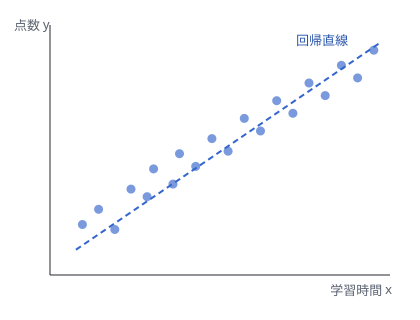
\includegraphics[width=0.6\textwidth]{figures/regression.svg}
\caption{正の相関をもつ散布図と回帰直線。点が右上がりの帯状に並んでいる。}
\end{figure}

\begin{quote}
\textbf{【演習】}\ 次のデータの相関係数を求めよ。
\[ (x, y) = (1, 2),\ (2, 3),\ (3, 5),\ (4, 4),\ (5, 6) \]
\end{quote}

\textbf{解答の指針:} \(\bar{x} = 3,\ \bar{y} = 4\)。分子 \(= (-2)(-2) + (-1)(-1) + 0 \cdot 1 + 1 \cdot 0 + 2 \cdot 2 = 9\)。分母 \(= \sqrt{10} \sqrt{10} = 10\)。よって \(r = 0.9\)。

\section{確率の基礎}

\subsection{確率の定義と性質}

試行の結果の全体を\textbf{標本空間} \(\Omega\) と呼び、事象は \(\Omega\) の部分集合です。すべての結果が同様に確からしいとき、事象 \(A\) の確率は
\[ P(A) = \frac{\#A}{\#\Omega} \]
確率の基本性質:
\begin{enumerate}
\item \(0 \le P(A) \le 1\), \(P(\Omega) = 1\)
\item \(P(\bar{A}) = 1 - P(A)\)(余事象)
\item \(P(A \cup B) = P(A) + P(B) - P(A \cap B)\)(加法定理)
\end{enumerate}

\subsection{条件付き確率と独立}

事象 \(B\) が起きたという条件のもとで \(A\) が起きる\textbf{条件付き確率}:
\[ P(A \mid B) = \frac{P(A \cap B)}{P(B)} \quad (P(B) > 0) \]
これを変形すると\textbf{乗法定理} \(P(A \cap B) = P(B)\, P(A \mid B)\) が得られます。\(P(A \mid B) = P(A)\) のとき、\(B\) の情報は \(A\) に影響せず、\(A\) と \(B\) は\textbf{独立}であるといいます。

\begin{quote}
\textbf{【例:ベイズの定理】}\ ある病気の検査は、病気があれば 99\% で陽性(感度 0.99)、なければ 5\% で誤って陽性(偽陽性率 0.05)。病気の有病率は 0.1\% とする。陽性の人が実際に病気である確率は?
\[ P(\text{病} \mid \text{陽}) = \frac{P(\text{陽} \mid \text{病}) P(\text{病})}{P(\text{陽})} = \frac{0.99 \times 0.001}{0.99 \times 0.001 + 0.05 \times 0.999} \approx 0.019 \]
わずか約 2\% です。まれな事象では偽陽性が圧倒するからで、ベイズの定理の有名な教訓です。
\end{quote}

\begin{quote}
\textbf{【演習】}\ 袋に白玉 3 個と赤玉 2 個が入っている。2 個を続けて取り出す(戻さない)。1 個目が白だったとき、2 個目も白である確率を求めよ。
\end{quote}

\textbf{解答の指針:} 条件付き確率で、白1個取り出し後の袋は白2赤2。よって \(2/4 = 1/2\)。

\section{確率変数と期待値}

\subsection{確率変数と確率分布}

結果を数値に対応させる関数が\textbf{確率変数}です。離散型なら各値 \(x\) に確率 \(p(x)\) を対応させる\textbf{確率質量関数}、連続型なら\textbf{確率密度関数} \(f(x)\) を使います。

\[ \text{(連続型)} \quad P(a \le X \le b) = \int_a^b f(x)\, dx, \qquad \int_{-\infty}^{\infty} f(x)\, dx = 1 \]

\subsection{期待値と分散}

\textbf{期待値}は「長期的な平均」で、確率で重みづけた平均です:
\[ E[X] = \sum_x x\, p(x) \quad \text{または} \quad E[X] = \int_{-\infty}^{\infty} x\, f(x)\, dx \]
\textbf{分散}は期待値まわりの2乗誤差の平均:
\[ V[X] = E[(X - E[X])^2] = E[X^2] - (E[X])^2 \]
この等式(計算しやすい形)は実務上、分散計算の定番です。

期待値と分散の基本法則(\(a, b\) は定数):
\[ E[aX + b] = a E[X] + b, \qquad V[aX + b] = a^2 V[X] \]
また独立な \(X, Y\) に対して
\[ E[X+Y] = E[X] + E[Y], \qquad V[X+Y] = V[X] + V[Y] \]
が成り立ちます。和の期待値は常に加法性をもつ一方、分散の加法性には\textbf{独立}が必要です。

\begin{quote}
\textbf{【例】}\ サイコロ \(X\) の期待値と分散。\(E[X] = \frac{1}{6}(1 + 2 + \cdots + 6) = 3.5\)。\(E[X^2] = \frac{1}{6}(1 + 4 + \cdots + 36) = \frac{91}{6}\)。よって \(V[X] = \frac{91}{6} - 3.5^2 = \frac{35}{12} \approx 2.92\)。
\end{quote}

\begin{quote}
\textbf{【演習】}\ \(X, Y\) は独立で \(E[X] = 2,\ V[X] = 4,\ E[Y] = -1,\ V[Y] = 1\) のとき、\(Z = 2X + Y + 3\) の期待値と分散を求めよ。
\end{quote}

\textbf{解答の指針:} \(E[Z] = 2 \cdot 2 + (-1) + 3 = 6\)。\(V[Z] = 2^2 \cdot 4 + 1 = 17\)。

\section{代表的な確率分布}

\subsection{二項分布}

成功確率 \(p\) の試行を独立に \(n\) 回行うときの成功回数 \(X\) は\textbf{二項分布} \(B(n, p)\) に従います:
\[ P(X = k) = \binom{n}{k} p^k (1-p)^{n-k}, \qquad E[X] = np, \qquad V[X] = np(1-p) \]
\(\binom{n}{k}\) は \(n\) 個から \(k\) 個選ぶ組合せの数で、成功位置の選び方を数えます。

\begin{quote}
\textbf{【例】}\ 表が出る確率 0.5 のコインを 10 回投げて表がちょうど 6 回出る確率:
\[ P(X = 6) = \binom{10}{6} 0.5^6 \cdot 0.5^4 = \frac{210}{1024} \approx 0.205 \]
\end{quote}

\subsection{ポアソン分布}

単位時間あたり平均 \(\lambda\) 回起きるまれな事象の発生回数は\textbf{ポアソン分布} Po(\(\lambda\)) に従います:
\[ P(X = k) = e^{-\lambda} \frac{\lambda^k}{k!}, \qquad E[X] = V[X] = \lambda \]
二項分布の \(n \to \infty,\ np \to \lambda\) の極限で現れます。コールセンターへの電話、1日あたりの事故件数、ページの誤字数などが古典的な例です。

\subsection{正規分布}

最も重要な連続分布が\textbf{正規分布} \(N(\mu, \sigma^2)\) です。密度関数は
\[ f(x) = \frac{1}{\sqrt{2\pi}\,\sigma} \exp\left( -\frac{(x - \mu)^2}{2\sigma^2} \right) \]
釣り鐘型の対称な形をします。\(\mu = 0, \sigma^2 = 1\) に標準化したものを\textbf{標準正規分布}といい、累積確率は数表や計算機で求めます。有名な値として
\[ P(-1 \le Z \le 1) \approx 0.683, \qquad P(-2 \le Z \le 2) \approx 0.954, \qquad P(-3 \le Z \le 3) \approx 0.997 \]
があり、これらは「68–95–99.7 ルール」としてデータの感覚を掴むのに役立ちます。

\begin{figure}[h]
\centering
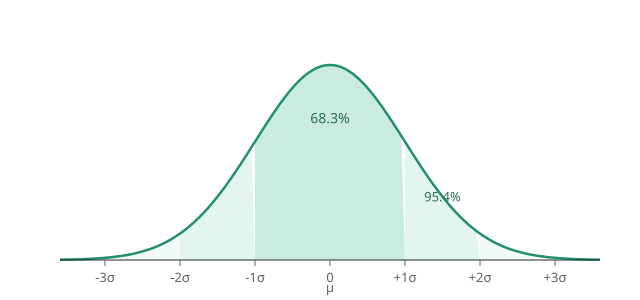
\includegraphics[width=0.85\textwidth]{figures/normal.svg}
\caption{標準正規分布の密度関数。平均から $\pm 1\sigma$ に約 68\%、$\pm 2\sigma$ に約 95\% が入る。}
\end{figure}

\begin{quote}
\textbf{【演習】}\ 身長が平均 170 cm、標準偏差 6 cm の正規分布に従うとする。身長が 182 cm を超える確率はおおよそいくらか。
\end{quote}

\textbf{解答の指針:} \(z = (182 - 170)/6 = 2\)。\(P(Z > 2) \approx 0.023\)。つまり上位約 2\%。

\section{標本と大数の法則}

\subsection{大数の法則}

標本平均 \(\bar{X}_n = \frac{1}{n} \sum X_i\) は、サンプル数 \(n\) を増やすと母平均 \(\mu\) に近づきます:
\[ \bar{X}_n \xrightarrow{p} \mu \quad (n \to \infty) \]
これが\textbf{大数の法則}です。カジノが長期的に必ず儲かるのも、保険が成立するのも、この法則の力です。

\subsection{中心極限定理}

推測統計の心臓部が\textbf{中心極限定理}( CLT )です。

\begin{quote}
\textbf{【定理:中心極限定理】}\ 平均 \(\mu\), 分散 \(\sigma^2\) の任意の分布に従う独立な確率変数 \(X_1, \dots, X_n\) に対して、\(n\) が大きいとき
\[ \bar{X}_n \approx N\left( \mu, \frac{\sigma^2}{n} \right), \qquad \text{すなわち} \quad Z = \frac{\bar{X}_n - \mu}{\sigma / \sqrt{n}} \approx N(0, 1) \]
\end{quote}

驚くべき点は\textbf{母集団の分布が何であってよい}ことです。元の分布がどんなに歪んでいても、平均をたくさん取れば標本平均は正規分布に近づきます。これにより、母集団の分布を知らなくても標本平均の誤差を正規分布で評価できます。

標本平均の標準偏差 \(\sigma/\sqrt{n}\) を\textbf{標準誤差}と呼びます。\(n\) を4倍すると誤差が半分になる——精度はサンプル数の平方根に比例してしか上がらない、という実務上非常に重要な帰結です。

\begin{quote}
\textbf{【演習】}\ 平均 500、標準偏差 100 の母集団から 100 個の標本を取る。標本平均が 520 を超える確率を求めよ。
\end{quote}

\textbf{解答の指針:} 標準誤差は \(100/\sqrt{100} = 10\)。\(z = (520 - 500)/10 = 2\) より \(P \approx 0.023\)。

\section{区間推定}

\subsection{点推定と区間推定}

母平均を「たぶんこの値」(点推定)でなく「この範囲に含まれる」(区間推定)で表します。標準正規分布の 95\% が \(-1.96\) から \(1.96\) に入ることを使うと、\(\sigma\) 既知のときの母平均 \(\mu\) の\textbf{95\% 信頼区間}は
\[ \bar{x} - 1.96 \frac{\sigma}{\sqrt{n}} \le \mu \le \bar{x} + 1.96 \frac{\sigma}{\sqrt{n}} \]

\textbf{信頼度 95\%} の意味の解釈が重要です。「この区間が 95\% の確率で \(\mu\) を含む」のではなく、「同じ手順で区間を作り続ければ、長期的に 95\% の区間が真の \(\mu\) を含む」という頻度論的な意味です。

\begin{quote}
\textbf{【例】}\ \(n = 64\), \(\bar{x} = 120\), \(\sigma = 16\) のとき
\[ 120 \pm 1.96 \times \frac{16}{8} = 120 \pm 3.92 \quad \Rightarrow \quad [116.08,\ 123.92] \]
\end{quote}

\(\sigma\) が未知で \(n\) が小さいときは、母標準偏差の推定値 \(s\) を使い、正規分布の代わりに\textbf{t 分布}を使います。t 分布は正規分布より裾が厚く、データが少ない不確実性を反映します。自由度 \(n-1\) の t 分布の 95\% 点 \(t_{n-1}\) で
\[ \bar{x} \pm t_{n-1} \frac{s}{\sqrt{n}} \]
とします。\(n\) が大きくなると t 分布は正規分布に収束します。

\begin{quote}
\textbf{【演習】}\ \(n = 25\), \(\bar{x} = 50\), \(s = 8\) のとき母平均の 95\% 信頼区間を求めよ。ただし自由度 24 の t 分布の 95\% 点は 2.064。
\end{quote}

\textbf{解答の指針:} \(50 \pm 2.064 \times 8/5 = 50 \pm 3.30\)、よって \([46.70,\ 53.30]\)。

\section{仮説検定}

\subsection{検定の枠組み}

\textbf{仮説検定}は「偶然だけでは説明できない差があるか」を判断する手続きです。

\begin{itemize}
\item \textbf{帰無仮説 \(H_0\)}: 「差はない」「効果はない」という有利な仮説。
\item \textbf{対立仮説 \(H_1\)}: 証明したい(調べたい)仮説。
\item \textbf{p 値}: \(H_0\) が正しいと仮定したとき、観測されたデータ以上に極端な結果が出る確率。
\end{itemize}

p 値があらかじめ決めた\textbf{有意水準} \(\alpha\)(慣習的に 0.05)より小さければ、\(H_0\) のもとでその結果は「偶然では説明しにくい」として \(H_0\) を棄却します。

\begin{quote}
\textbf{【注意】}\ p 値は \(H_0\) が正しい確率ではありません。「\(H_0\) を棄却できなかった」は「\(H_0\) が正しい」の証明でもありません(単に証拠が足りないだけ)。また有意水準ぎりぎりの判断に意味はなく、効果の大きさ(効果量)と一緒に報告するのが現代の標準です。
\end{quote}

\subsection{母平均の z 検定}

\(\sigma\) 既知のとき、統計量
\[ Z = \frac{\bar{x} - \mu_0}{\sigma / \sqrt{n}} \]
が \(H_0: \mu = \mu_0\) のもとで標準正規分布に従うことを使います。

\begin{quote}
\textbf{【例】}\ ある工場の製品の重さは平均 \(\mu_0 = 500\) g とされてきた。新しい製法で \(n = 100\) 個測ったところ \(\bar{x} = 505\) g。母標準偏差は 20 g と既知。重さが変わったといえるか(両側検定、\(\alpha = 0.05\))。
\[ Z = \frac{505 - 500}{20/\sqrt{100}} = \frac{5}{2} = 2.5 \]
標準正規の棄却域は \(|Z| > 1.96\) なので \(H_0\) を棄却。新しい製法で重さは変化したと結論できる(p 値 \(\approx 0.012\))。
\end{quote}

\subsection{検定の2種の過誤}

\begin{quote}
\textbf{【定理:2種の過誤】}
\begin{enumerate}
\item \textbf{第1種の過誤}: \(H_0\) が正しいのに棄却してしまう(無実の人を有罪にする)。確率は \(\alpha\)。
\item \textbf{第2種の過誤}: \(H_0\) が誤りなのに棄却できない(犯人を見逃す)。確率は \(\beta\)。
\end{enumerate}
\end{quote}

\(1 - \beta\) を\textbf{検出力}といい、真の効果があったときにそれを見つけられる確率です。標本数を増やすほど検出力は上がります。「なぜ \(n = 30\) くらい必要なのか」の答えは、所定の検出力を確保するサンプルサイズ設計にあります。

\begin{quote}
\textbf{【演習】}\ 両側検定で \(z = 2.1\) を得た。p 値はおよそいくらか(\(P(Z > 2.1) \approx 0.0179\))。\(\alpha = 0.05\) での結論は?
\end{quote}

\textbf{解答の指針:} 両側なので p 値 \(= 2 \times 0.0179 \approx 0.036 < 0.05\)。帰無仮説を棄却する。

\section{回帰分析}

\subsection{最小2乗法}

\(x\) から \(y\) を予測する直線 \(y = a + bx\) を、残差の2乗和
\[ S(a, b) = \sum_{i=1}^{n} (y_i - a - b x_i)^2 \]
を最小にするように選ぶのが\textbf{最小2乗法}です。\(\partial S / \partial a = \partial S / \partial b = 0\) とおいて解くと
\[ b = \frac{\sum (x_i - \bar{x})(y_i - \bar{y})}{\sum (x_i - \bar{x})^2} = r \frac{s_y}{s_x}, \qquad a = \bar{y} - b \bar{x} \]
回帰係数 \(b\) は相関係数と \(s_y / s_x\) の積になっています。相関が強いほど、また \(y\) のばらつきに比べて \(x\) のばらつきが小さいほど、傾きは急になります。

\begin{quote}
\textbf{【例】}\ 学習時間 \(x\) と点数 \(y\) のデータで \(\bar{x} = 4,\ \bar{y} = 60,\ r = 0.8,\ s_x = 1.5,\ s_y = 10\) のとき
\[ b = 0.8 \times \frac{10}{1.5} \approx 5.33, \qquad a = 60 - 5.33 \times 4 \approx 38.7 \]
回帰直線は \(y = 38.7 + 5.33 x\)。1時間勉強するごとに約 5.3 点上がる、という読み方。
\end{quote}

\subsection{決定係数}

回帰直線がデータのばらつきをどれだけ説明するかを\textbf{決定係数}で測ります:
\[ R^2 = r^2 \]
たとえば \(r = 0.8\) なら \(R^2 = 0.64\) で、「\(y\) のばらつきの 64\% を \(x\) で説明した」と読みます。

\begin{quote}
\textbf{【注意:外挿の危険】}\ 回帰直線はデータの観測範囲での関係を表すもので、範囲外に無批判に延長してはいけません。学習時間 2〜6 時間のデータから「10 時間勉強すれば 92 点」と予測するのは外挿であり、関係の形が範囲外で変わっている可能性を無視しています。
\end{quote}

\begin{quote}
\textbf{【演習】}\ \(r = -0.5\) のとき、\(y\) のばらつきの何\% を \(x\) で説明するか。
\end{quote}

\textbf{解答の指針:} \(R^2 = 0.25\)、つまり 25\%。

\section{実データで学ぶ — 手を動かす統計}

この節では、20 人分の小さなテスト得点データを実際に集計し、Python コードで確かめます。本編の公式が「計算の手順」ではなく「問いへの答え方」として使えるようになるのが狙いです。

\subsection{データを眺める}

あるクラス 20 人の算数テスト(100 点満点)の得点が次の通りでした。

\begin{center}
\begin{tabular}{|cccccccccc|}
\hline
55 & 62 & 64 & 68 & 70 & 72 & 74 & 75 & 78 & 80 \\
82 & 84 & 85 & 88 & 90 & 92 & 94 & 96 & 98 & 55 \\
\hline
\end{tabular}
\end{center}

まず 2 人が 55 点(うち 1 人は欠席による再テスト)という分布の端に注目します。平均は
\[ \bar{x} = \frac{1}{20} \sum x_i = 77.35 \]
です。中央値は並べ替えた 10 番目と 11 番目の平均で \(\frac{80 + 82}{2} = 81\)。平均より中央値のほうが大きく、分布が左(低得点側)に引っ張られていることが分かります。

\subsection{Python で確かめる}

同じ集計を Python で書くと次のようになります。

\begin{lstlisting}[language=Python]
import statistics

scores = [55, 62, 64, 68, 70, 72, 74, 75, 78, 80,
          82, 84, 85, 88, 90, 92, 94, 96, 98, 55]

print(statistics.mean(scores))     # 77.35
print(statistics.median(scores))   # 81.0
print(statistics.stdev(scores))    # 13.0 (標本標準偏差)
print(statistics.quantiles(scores, n=4))  # 四分位点
\end{lstlisting}

標準偏差(不偏推定値)は約 13 点。つまり「平均 77 点、±13 点の範囲におおよそ半分以上の生徒」が入ります。四分位点から IQR を計算すれば箱ひげ図が描け、再テストの 55 点が外れ値候補かどうかも判定できます。

\subsection{母集団への推測}

この 20 人を「標本」として、より大きな集団(たとえば同年度の全 5 クラス)の平均を推定してみます。\(n = 20\), \(\bar{x} = 77.35\), 標本標準偏差 \(s \approx 13.0\) から、母平均の 95\% 信頼区間は
\[ 77.35 \pm t_{19} \times \frac{13.0}{\sqrt{20}} \]
で、自由度 19 の t 分布の 95\% 点は 2.093 なので
\[ 77.35 \pm 2.093 \times 2.91 = 77.35 \pm 6.09 \quad \Rightarrow \quad [71.3,\ 83.4] \]
となります。「20 人から ±6 点の精度で全体の平均が言える」という感覚、そして**精度は \(\sqrt{n}\) にしか比例しない**という制約を実データの手ざわりで掴むのが、この節の到達点です。

\begin{quote}
\textbf{【演習】}\ 上のデータから欠席再テストの 55 点を除外した 19 人で同じ計算をし、平均と標準偏差がどう変わるか確かめよ。外れ値 1 件が区間推定をどれだけ動かすかを観察せよ。
\end{quote}

\textbf{解答の指針:}\ 19 人の平均は約 78.6、標準偏差は約 11.6 に縮む。標準誤差は \(11.6/\sqrt{19} \approx 2.66\) で区間も \([73.0,\ 84.2]\) と狭まる。外れ値の扱いが推定に実害を与える具体例。

\section{おわりに — 統計的思考の作法}

この教科書で学んだ流れを振り返ります。

\textbf{記述統計}(平均・分散・相関)は手元のデータを忠実に要約する技術です。\textbf{確率論}は偶然の数学的モデルを与えます。そして\textbf{推測統計}(標本分布・区間推定・検定・回帰)は、確率のモデルを逆向きに使い、データから母集団についての結論を引き出します。中心極限定理がその橋渡しの核心でした。

実データに向き合うときの作法を最後にまとめます。

\begin{enumerate}
\item \textbf{データの由来を確認する}: 標本が母集団を代表しているか。偏ったサンプルからの推測は無効です。
\item \textbf{まず図を描く}: ヒストグラムと散布図が、代表値や相関係数の計算より先に歪み・外れ値・非線形性を教えてくれます。
\item \textbf{誤差を報告する}: 点推定だけではなく信頼区間を、差だけではなく効果量と検出力を添える。
\item \textbf{因果と相関を区別する}: 相関があっても因果の方向や交絡の有無は別の議論(実験設計、因果推論)を必要とします。
\end{enumerate}

\begin{quote}
\textbf{【総合演習】}
\begin{enumerate}
\item 平均 120、標準偏差 15 の分布に従う検査得点で、得点 150 以上の割合を求めよ。
\item \(n = 36\) の標本で \(\bar{x} = 47\), \(s = 9\)。母平均の 95\% 信頼区間を求めよ(自由度 35 の t 値は 2.030)。
\item 帰無仮説のもとで p 値 0.03 が出た。これが「帰無仮説が正しい確率が 3\%」ではない理由を2つ挙げよ。
\end{enumerate}
\end{quote}

\textbf{解答の指針:} 1. \(z = 2\) より約 2.3\%。2. \(47 \pm 2.030 \times 9/6 = 47 \pm 3.05\)、よって \([43.95,\ 50.05]\)。3. p 値は「\(H_0\) のもとでデータ以上に極端な結果の確率」であり条件の向きが逆であること、実際に 3\% に寄与するのは \(H_0\) が真の事前確率(有病率に相当)と検出力の兼ね合いであること(ベイズの定理の例題参照)。

\end{document}
